% XeLaTeX; editable vector plot.
\documentclass[UTF8]{ctexart}
\usepackage[a4paper,margin=20mm]{geometry}
\usepackage{fontspec,pgfplots,caption}
\pgfplotsset{compat=1.18}
\setmainfont{Times New Roman}
\pagestyle{empty}
\definecolor{curveblue}{HTML}{287FA1}
\definecolor{curveorange}{HTML}{EF8A32}
\begin{document}\begin{figure}[ht]\centering
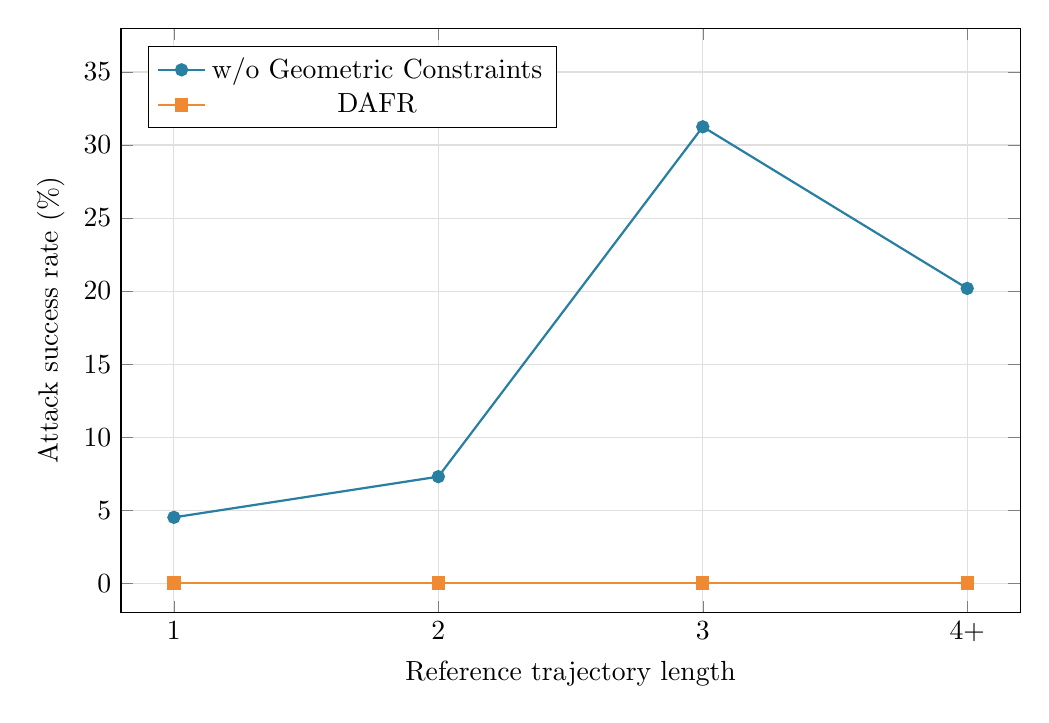
\begin{tikzpicture}\begin{axis}[width=13cm,height=9cm,xmin=.8,xmax=4.2,ymin=-2,ymax=38,
xtick={1,2,3,4},xticklabels={1,2,3,4+},ytick={0,5,...,35},grid=major,grid style={gray!25},
xlabel={Reference trajectory length},ylabel={Attack success rate (\%)},legend pos=north west,
cycle list={{curveblue},{curveorange}}]
\addplot+[thick,mark=*] coordinates {(1,4.50450450) (2,7.29166667) (3,31.25000000) (4,20.18348624)};\addlegendentry{w/o Geometric Constraints}
\addplot+[thick,mark=square*] coordinates {(1,0.00000000) (2,0.00000000) (3,0.00000000) (4,0.00000000)};\addlegendentry{DAFR}
\end{axis}\end{tikzpicture}
\caption{AgentDojo 中几何约束的安全收益与参考轨迹长度。采用 DeepSeek V4 Flash 的归档消融记录，按官方参考解的工具调用数分为 1、2、3、至少 4 步；每组分别包含 10、20、9、32 个用户任务，对应 111、192、64、218 次攻击执行，两个配置使用相同任务与攻击。ASR 按组内攻击执行记录求平均。去掉几何约束时，各组 ASR 为 4.5\%、7.3\%、31.2\%、20.2\%；完整 DAFR 各组均为 0\%。这是一项跨任务的长度分组分析，各组领域与任务组成不同，不表示只增加步骤就会产生同等幅度的变化。}
\end{figure}\end{document}
